\documentclass[10pt,a4paper,titlepage]{report}
\usepackage[utf8]{inputenc}
\usepackage{amsmath}
\usepackage{amsfonts}
\usepackage{amssymb}
\usepackage{graphicx}
\usepackage{xcolor}
\usepackage{minted}


\nonstopmode
\begin{document}
\begin{titlepage}
		\author{Rwithik Manoj\\Roll No. 53\\TVE17CS054}
\title{Foss Lab}
\date{\today}
\maketitle
\end{titlepage}

\chapter*{Problem 1}

\section*{Problem Statement}

Write a bash script to find the binary equivalent of a given number.

\section*{Theory}

A decimal numbers binary equvalent can be found by repeatedlt prepending the remainder after dividing the number by 2. 

\section*{Implementation}

The script reads the decimal number into a variable a and declares the variable b as an empty string. Then it loops as long as a is greater than 0. In each iteration, it prepend the remainder after dividing a by 2 and then divides a by 2 using floor division. This is more effecient than appending the remainder and then reversing the string with another loop. 

\section*{Test Runs}

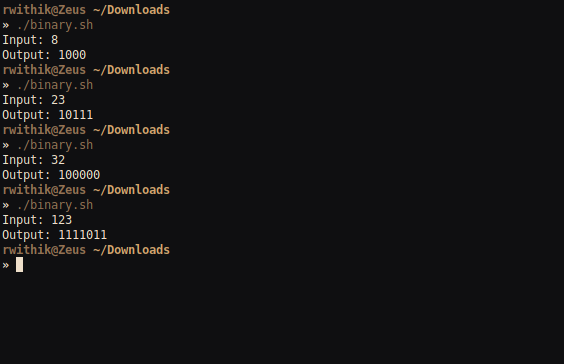
\includegraphics[width=\linewidth]{../Images/ExamReport/binary.png}

\section*{Code}

\inputminted[tabsize=4]{bash}{../Scripts/Exam/binary.sh}

\chapter*{Problem 2}

\section*{Problem Statement}

Given a file containing the marks obtained by students for 3 subjects in an
exam. In order to pass, student should score at least 50 marks in every
subject. The file has one record(line) for each student in the following
format:\newline
roll\_number subject1 subject2 subject3

\section*{Theory}

Read the file with awk. Check if all the marks of a roll number are at least 50. If it is, print ``pass'', else print ``fail''.

\section*{Implementation}

The implementation is simple. An if condition checks if all the marks are greater than 50 or not and print the appropriate result. 

\section*{Test Runs}

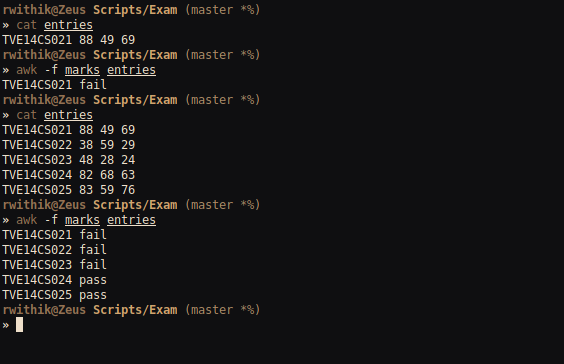
\includegraphics[width=\linewidth]{../Images/ExamReport/marks.png}

\section*{Code}

\inputminted[tabsize=4]{bash}{../Scripts/Exam/marks}

\chapter*{Problem 3}

\section*{Problem Statement}

Implement PHP application that asks a random question(from a given set) to
the user and evaluates if the user’s answer is correct.

\section*{Theory}

There is a file with all the questions and answers. Read all the questions and answers from the file and choose a random question to display. Check if the answer submitted by the user is correct and display the corrosponding message.

\section*{Implementation}

The questions.php file checks if the session item storing the questions or the one storing the answers is empty. It any of them are empty, then it read the questions and answers from the file and inserts them into the session items. 

The form sends a post request to the same file where the answer entered by the user is compared to the answer entered by the user and the correct answer. If they match, the user is redirected to the success.php file after setting a session variable named success. 

In the success.php file, the success session variable is checked and if it is set, the message is displayed. Otherwise the user is redirected to the questions.php file.

\section*{Code}

\subsection*{questions.php}

\inputminted[tabsize=4]{php}{../Scripts/Exam/questions.php}

\subsection*{success.php}

\inputminted[tabsize=4]{php}{../Scripts/Exam/success.php}

\end{document}
